\documentclass[10pt]{article}
\usepackage[utf8]{inputenc}
\usepackage[includehead, headheight=10mm, margin=15mm ]{geometry}
\usepackage{amsmath}
\usepackage{amsthm}
\usepackage{amsfonts}
\usepackage{xcolor}
\usepackage{graphicx}
\usepackage{titling}
\usepackage{fancyhdr}
\usepackage{listings}
\usepackage{hyperref}

\title{APPM 4600 Lab 8}
\author{Edward Wawrzynek}
\date{17 October 2024}

\newcommand*{\dif}{\mathop{}\!\mathrm{d}}

\makeatletter
\def\@maketitle{%
  \newpage
  \null
  \vskip 1em%
  \begin{center}%
  \let \footnote \thanks
    {\LARGE \@title \par}%
    \vskip 1em%
    {\normalfont \@date}
  \end{center}%
  \par
  \vskip 1em}
\makeatother

\begin{document}

\pagestyle{fancy}
    \fancyhf{} % clear all header and footer fields
    \fancyhead[L]{\thetitle}
    \fancyhead[R]{\theauthor}

\makeatletter
\begin{center}
    {\Large \@title}
    \vskip 1mm
    {\normalfont \@date}
    \vskip 1em
\end{center}
\makeatother

The code for this lab can be seen at the end of this document, or on github \href{https://github.com/edwardwawrzynek/APPM4600/blob/master/Labs/Lab\%208/demo_linspline.py}{here} (linear splines) and \href{https://github.com/edwardwawrzynek/APPM4600/blob/master/Labs/Lab\%208/demo_cubicspline.py}{here} (cubic splines).

\section{Prelab}
\begin{enumerate}
  \item The code to evaluate a line through given points is included at the end of the document, in the function \texttt{eval\_line}.
\end{enumerate}

\section{Linear Splines}
\begin{enumerate}
  \item The code for the linear splines was implemented. Shown below is the interpolation of the function \begin{align*}
      f(x) = \frac{1}{1+(10*x)^2}
  \end{align*} with various numbers of interpolation points distributed uniformly over the interval \(x \in [-1, 1]\).

  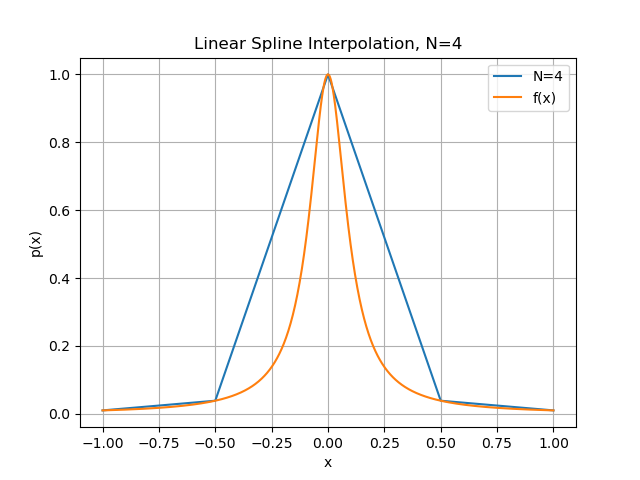
\includegraphics[width=0.49\textwidth]{lin4.png}
  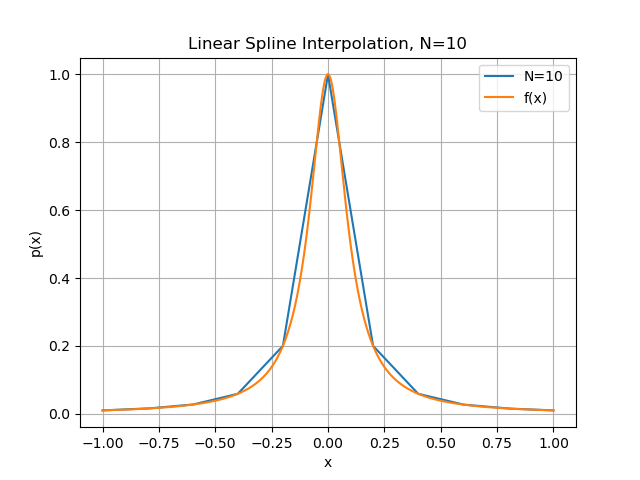
\includegraphics[width=0.49\textwidth]{lin10.png}
  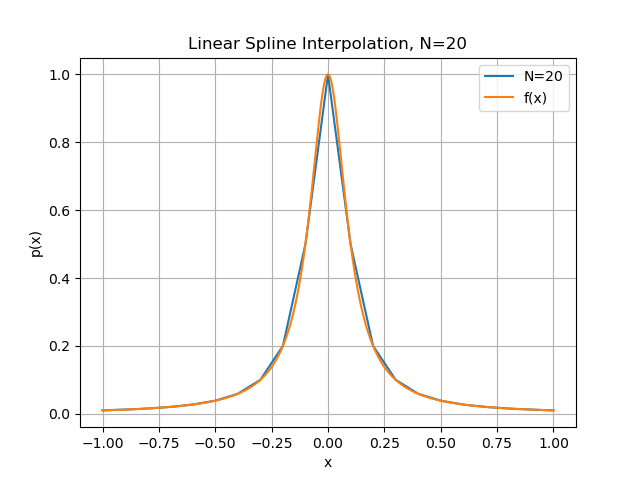
\includegraphics[width=0.49\textwidth]{lin20.png}
  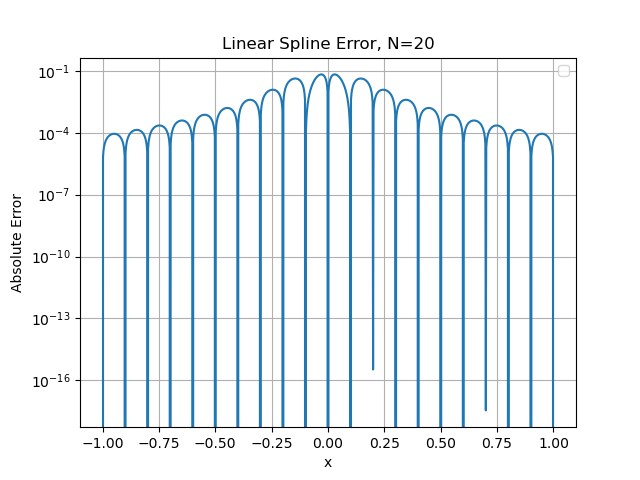
\includegraphics[width=0.49\textwidth]{lin_error20.png}

  Notice that the spline interpolation does not display the Runge phenomenon.

\end{enumerate}

\section{Cubic Splines}
\begin{enumerate}
  \item The code for the cubic splines was implemented. Shown below is the interpolation of the same function as the previous section.
  
  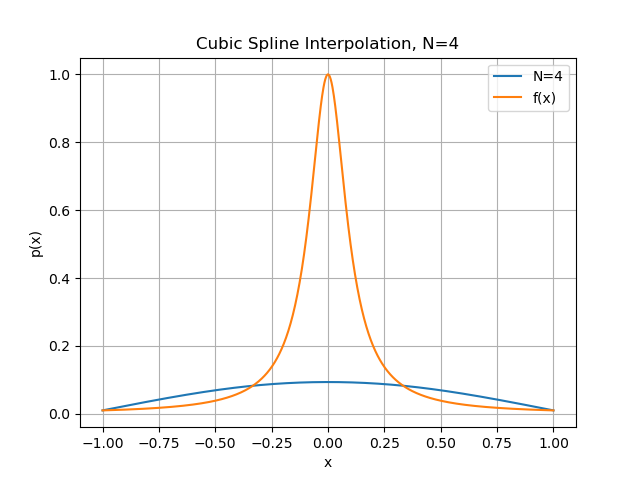
\includegraphics[width=0.49\textwidth]{cubic4.png}
  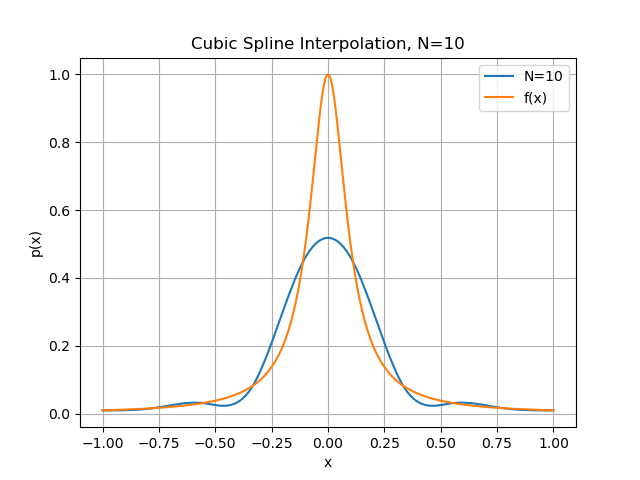
\includegraphics[width=0.49\textwidth]{cubic10.png}
  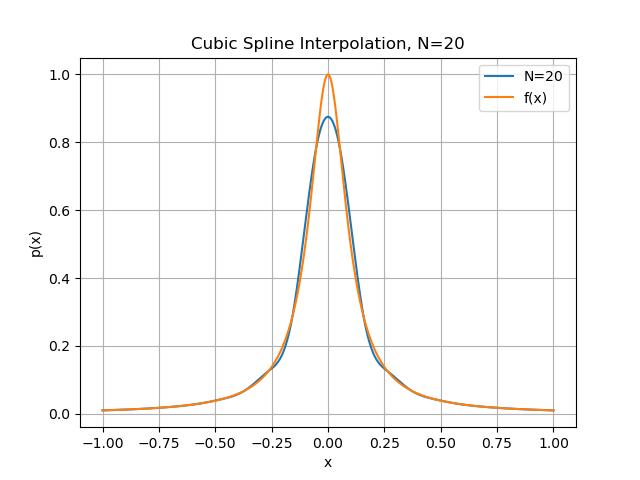
\includegraphics[width=0.49\textwidth]{cubic20.png}
  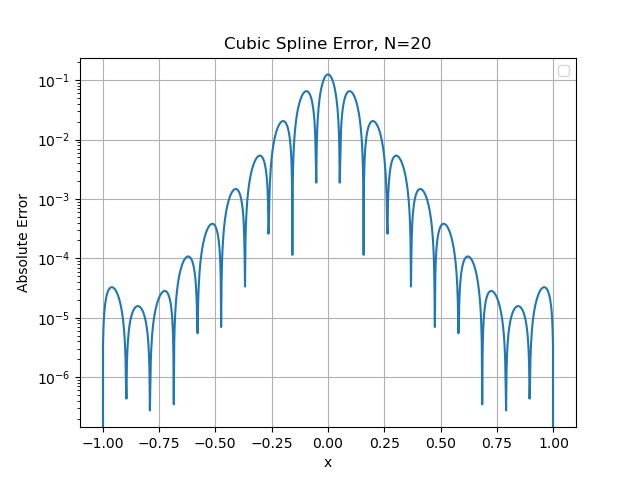
\includegraphics[width=0.49\textwidth]{cubic_error20.png}

  Notice that the cubic interpolation displays similar error as the linear interpolation, through slightly lower for \(x\) near 1 or -1. As before, it does not display the Runge phenomenon.
\end{enumerate}

\section{Linear Splines Code}
{\small \lstinputlisting[language=Python]{demo_linspline.py}}

\section{Cubic Splines Code}
{\small \lstinputlisting[language=Python]{demo_cubicspline.py}}    

\end{document}
